\documentclass{beamer}
\usetheme{Madrid}
\usecolortheme{seahorse}
\usepackage{amsmath}
\usepackage{amssymb}
\usepackage{graphicx}
\usepackage{tikz}
\usepackage{chemfig}

\title{Chemical Oscillator Systems}
\subtitle{Exploring Cyclic Behavior in Reaction Networks}
\author{Chemical Dynamics Analysis}
\date{\today}

\begin{document}

\begin{frame}
\titlepage
\end{frame}

\begin{frame}{Outline}
\tableofcontents
\end{frame}

\section{Introduction}

\begin{frame}{Chemical Oscillators}
\begin{itemize}
    \item Chemical reactions that exhibit periodic behavior
    \item Require:
    \begin{itemize}
        \item Nonlinear kinetics
        \item Feedback mechanisms
        \item Energy/mass flow (open system)
    \end{itemize}
    \item Examples in nature:
    \begin{itemize}
        \item Belousov-Zhabotinsky reaction
        \item Glycolytic oscillations
        \item Circadian rhythms
    \end{itemize}
\end{itemize}
\end{frame}

\section{Brusselator System}

\begin{frame}{Brusselator Model}
\begin{block}{Reaction Scheme}
\begin{align}
A &\xrightarrow{a} X \\
2X + Y &\xrightarrow{} 3X \quad \text{(autocatalytic)} \\
B + X &\xrightarrow{b} Y + D \\
X &\xrightarrow{} E \quad \text{(decay)} \\
Y &\xrightarrow{} Z \quad \text{(slow conversion)} \\
Z &\xrightarrow{} \text{recycle}
\end{align}
\end{block}

\begin{itemize}
    \item Classic model for chemical oscillations
    \item Demonstrates Hopf bifurcation
    \item Parameters: $a = 1.0$, $b = 3.0$
\end{itemize}
\end{frame}

\begin{frame}{Brusselator ODEs}
\begin{block}{System of Differential Equations}
\begin{align}
\frac{dX}{dt} &= a - (b+1)X + X^2Y - 0.1X \\
\frac{dY}{dt} &= bX - X^2Y - 0.05Y \\
\frac{dZ}{dt} &= 0.05Y - 0.1Z
\end{align}
\end{block}

\begin{itemize}
    \item Nonlinear term: $X^2Y$ (autocatalysis)
    \item Fixed point loses stability when $b > 1 + a^2$
    \item For our parameters: $3.0 > 1 + 1.0^2 = 2.0$
\end{itemize}
\end{frame}

\begin{frame}{Brusselator Dynamics}
\begin{columns}
\begin{column}{0.5\textwidth}
\begin{itemize}
    \item \textbf{Limit Cycle}: Stable periodic orbit
    \item All trajectories converge to the cycle
    \item Period $\approx 7.4$ time units
    \item Amplitude depends on parameters
\end{itemize}
\end{column}
\begin{column}{0.5\textwidth}
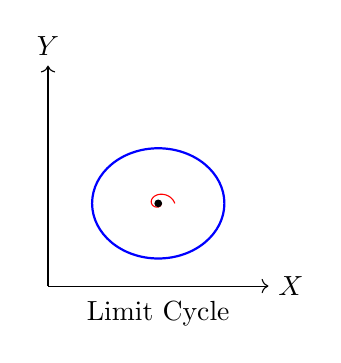
\begin{tikzpicture}[scale=0.7]
    % Draw axes
    \draw[->] (0,0) -- (4,0) node[right] {$X$};
    \draw[->] (0,0) -- (0,4) node[above] {$Y$};
    
    % Draw limit cycle
    \draw[thick, blue] (2,1.5) ellipse (1.2 and 1);
    
    % Draw spiral
    \draw[red, domain=0:720, samples=100, smooth] 
        plot ({2+0.3*exp(-\x/200)*cos(\x)}, 
              {1.5+0.25*exp(-\x/200)*sin(\x)});
    
    % Fixed point
    \fill (2,1.5) circle (2pt);
    
    \node at (2,-0.5) {Limit Cycle};
\end{tikzpicture}
\end{column}
\end{columns}
\end{frame}

\section{Cyclic Reaction System}

\begin{frame}{Cyclic Reaction Network}
\begin{block}{Reaction Scheme}
\begin{align}
A + B &\xrightarrow{k_1} 2B \quad \text{(A catalyzes B)} \\
B + C &\xrightarrow{k_2} 2C \quad \text{(B catalyzes C)} \\
C &\xrightarrow{k_6} A \quad \text{(C recycles to A)} \\
C &\xrightarrow{k_3} \text{decay} \\
A + C &\rightleftharpoons AC \quad \text{(stabilizing)}
\end{align}
\end{block}

\begin{itemize}
    \item Inspired by predator-prey dynamics
    \item Cyclic catalysis: A → B → C → A
    \item Each species catalyzes the next
\end{itemize}
\end{frame}

\begin{frame}{Cyclic System ODEs}
\begin{block}{Differential Equations}
\begin{align}
\frac{dA}{dt} &= -k_1 AB + k_6 C - k_4 AC + k_5 AC_{eq} \\
\frac{dB}{dt} &= k_1 AB - k_2 BC \\
\frac{dC}{dt} &= k_2 BC - k_3 C - k_6 C
\end{align}
\end{block}

\begin{itemize}
    \item Rate constants:
    \begin{itemize}
        \item $k_1 = 0.1$ (A+B → 2B)
        \item $k_2 = 0.15$ (B+C → 2C)
        \item $k_3 = 0.05$ (C decay)
        \item $k_6 = 0.08$ (C → A)
    \end{itemize}
\end{itemize}
\end{frame}

\section{Phase Space Analysis}

\begin{frame}{Phase Portraits}
\begin{columns}
\begin{column}{0.5\textwidth}
\textbf{2D Projection}
\begin{itemize}
    \item Vector field shows flow
    \item Trajectories form closed orbits
    \item Nullclines intersect at fixed points
\end{itemize}
\end{column}
\begin{column}{0.5\textwidth}
\textbf{3D Phase Space}
\begin{itemize}
    \item Full system dynamics
    \item Vector field on Z-slices
    \item Reveals 3D structure of limit cycle
\end{itemize}
\end{column}
\end{columns}

\vspace{0.5cm}
\begin{center}
\includegraphics[width=0.8\textwidth]{chemical_oscillator_analysis.pdf}
\end{center}
\end{frame}

\begin{frame}{Mathematical Analysis}
\begin{block}{Stability Analysis}
\begin{itemize}
    \item Linearization around fixed point: $\mathbf{J} = \frac{\partial \mathbf{f}}{\partial \mathbf{x}}$
    \item Eigenvalues determine stability
    \item Complex eigenvalues → oscillations
    \item Positive real part → growing oscillations
\end{itemize}
\end{block}

\begin{block}{Conservation Properties}
\begin{itemize}
    \item Neither system strictly conserves mass
    \item Energy input required for oscillations
    \item Brusselator: constant input of A and B
    \item Cyclic: autocatalysis violates conservation
\end{itemize}
\end{block}
\end{frame}

\section{Comparison}

\begin{frame}{System Comparison}
\begin{table}
\centering
\begin{tabular}{|l|c|c|}
\hline
\textbf{Property} & \textbf{Brusselator} & \textbf{Cyclic} \\
\hline
Oscillation type & Limit cycle & Periodic/quasi-periodic \\
Period & $\approx 7.4$ & Variable \\
Stability & Globally stable & Depends on parameters \\
Bifurcation & Hopf at $b = 1 + a^2$ & Complex \\
Physical basis & Abstract & Predator-prey like \\
\hline
\end{tabular}
\end{table}

\begin{block}{Key Differences}
\begin{itemize}
    \item Brusselator: Well-studied, predictable
    \item Cyclic: More complex dynamics, multiple timescales
    \item Both require open systems (mass/energy flow)
\end{itemize}
\end{block}
\end{frame}

\section{Applications}

\begin{frame}{Real-World Examples}
\begin{columns}
\begin{column}{0.5\textwidth}
\textbf{Biological Oscillators}
\begin{itemize}
    \item Circadian rhythms
    \item Cell cycle
    \item Calcium oscillations
    \item Neural activity
\end{itemize}
\end{column}
\begin{column}{0.5\textwidth}
\textbf{Chemical Systems}
\begin{itemize}
    \item BZ reaction
    \item pH oscillators
    \item Enzyme reactions
    \item Electrochemical oscillations
\end{itemize}
\end{column}
\end{columns}

\vspace{0.5cm}
\begin{block}{Design Principles}
\begin{itemize}
    \item Positive feedback (autocatalysis)
    \item Negative feedback (inhibition/decay)
    \item Time delays
    \item Nonlinear kinetics
\end{itemize}
\end{block}
\end{frame}

\section{Conclusions}

\begin{frame}{Summary}
\begin{itemize}
    \item Chemical oscillators exhibit rich dynamics
    \item Key requirements:
    \begin{itemize}
        \item Nonlinearity
        \item Feedback loops
        \item Open system
    \end{itemize}
    \item Mathematical tools:
    \begin{itemize}
        \item Phase portraits
        \item Stability analysis
        \item Bifurcation theory
    \end{itemize}
    \item Applications span chemistry, biology, and physics
\end{itemize}

\begin{block}{Future Directions}
\begin{itemize}
    \item Coupled oscillators
    \item Stochastic effects
    \item Spatial patterns
    \item Control strategies
\end{itemize}
\end{block}
\end{frame}

\begin{frame}{References}
\begin{thebibliography}{9}
\bibitem{prigogine} 
I. Prigogine and R. Lefever,
\textit{Symmetry Breaking Instabilities in Dissipative Systems},
J. Chem. Phys. 48, 1695 (1968).

\bibitem{strogatz} 
S.H. Strogatz,
\textit{Nonlinear Dynamics and Chaos},
Westview Press (2014).

\bibitem{epstein} 
I.R. Epstein and J.A. Pojman,
\textit{An Introduction to Nonlinear Chemical Dynamics},
Oxford University Press (1998).

\bibitem{murray} 
J.D. Murray,
\textit{Mathematical Biology},
Springer-Verlag (2002).
\end{thebibliography}
\end{frame}

\end{document}
